\documentclass[12pt]{article}
\usepackage{lipsum}
\usepackage{amsmath, amssymb}
\usepackage[margin=2cm]{geometry} % Margin
\usepackage{float} % Allows you to control float positions
\usepackage{graphicx} % Allows you to import images
\usepackage{multirow}
\usepackage[myheadings]{fullpage}
\usepackage{fancyhdr}
\usepackage{lastpage}
\usepackage{array}
\usepackage{amsmath}
% !TeX spellcheck = en_AU
\usepackage{listings}
\usepackage{xcolor} % for setting colors
\usepackage{cite}
\usepackage{algorithm}
\usepackage{algorithmic}

\newcommand{\HRule}[1]{\rule{\linewidth}{#1}}
\setcounter{tocdepth}{5}
\setcounter{secnumdepth}{5}


% set the default code style
\lstset{
	frame=tb, % draw a frame at the top and bottom of the code block
	tabsize=4, % tab space width
	showstringspaces=false, % don't mark spaces in strings
	numbers=left, % display line numbers on the left
	commentstyle=\color{green}, % comment color
	keywordstyle=\color{blue}, % keyword color
	stringstyle=\color{red}, % string color
	breaklines=true, % wrapping the lines back around
	postbreak=\mbox{\textcolor{red}{$\hookrightarrow$}\space} % Annotating the wrapped lines
}


\newcolumntype{L}[1]{>{\raggedright\let\newline\\\arraybackslash\hspace{0pt}}m{#1}}

%-------------------------------------------------------------------------------
% HEADER & FOOTER
%-------------------------------------------------------------------------------
\usepackage{fancyhdr}
\pagestyle{fancy}
\fancyhead{}
\renewcommand{\headrulewidth}{0pt}
\renewcommand{\footrulewidth}{0pt}

\title{Assignment 1 - Problem Solving Task}

\author{Jeremiah Dufourq}
\begin{document}
\begin{titlepage}
	\centering
	
	
	{\scshape\LARGE Queensland University of Technology \par}
	\vspace{5cm}
	{\scshape\Large Implementation of a Brute Force algorithm to find the median of an array\par}
	\vspace{1.5cm}
	{\huge\bfseries CAB301\par}
	\vspace{2cm}
	{\Large\itshape Jeremiah Dufourq n9960651\par}
	
	% Bottom of the page
	{\large \today\par}
\end{titlepage}


\newpage
\tableofcontents
\newpage

\section{Executive Summary:}
The Brute Force approach to solving problems in algorithmic design is the simplest of all algorithm design approaches. It seeks to solve a problem by iterating through all possible combinations of the algorithm. Hence, through this process, the Brute Force approach arrives at the solution. A formal definition is noted below from, \textit{An Introduction to the Design and Analysis of Algorithms}, by \textit{Anany Levitin} \cite{RN1}
\begin{quotation}
	\textit{“Brute force is a straight forward approach to solving a problem, usually directly based on the problem statement and definitions of the concepts involved.”}
	
\end{quotation}

Whilst this is a straight forward method to apply, in practice there are a few issues with it. One of the major issues is the efficiency of the algorithm, which is hindered depending on the problem. Because this approach iterates through all combinations of the problem, its efficiency is the product of all possible outcomes of the problem.

This report will analyse the implementation of the \textbf{\textit{BruteForceMedian}} algorithm through empirical analysis. A detailed description of the algorithm will be discussed in terms of its time complexity, average, worst and best cases efficiencies. The implementation of the algorithm through pseudocode and C++ will be outline, as well as the design of the experiments regarding the functionality, number of operations and time efficiency. The results from each of the tests will be interpreted, analysed and compared to the theoretical complexity of the algorithm.

\newpage 
	
\section{Description of algorithm:}
The \textit{\textbf{BruteForceMedian}} algorithm can be described succinctly as an algorithm which takes half the array as a rounded value $(k)$ and compares each element in the array to each other. If the elements are equal to each other, it increments a \textit{numequal} variable by 1. If one of the elements is smaller than the other, it increments a \textit{numsmaller} variable by 1. It repeats these steps until the \textit{numsmaller} is less than $(k)$ and \textit{numequal} and \textit{numsmaller }are less than or equal to $(k)$ then it returns the element at that location in the array. In this case, it compares each element in the array up to half of the array size (see listing \ref{lst:BruteForceMedian}).

\begin{lstlisting}[caption={BruteForceMedian algorithm implementation (timing implementation)},label={lst:BruteForceMedian},language=C++]
int BruteForceMedianTime(vector<int> &A)
{
	// Calculate the half-way index of the array.
	size_t size = A.size(); // Storing the size as size_t (unsigned int)
	int k = (int) ceil(size/ 2.0);
	
	for (int i = 0; i <= (A.size()-1); i++) {
		int numSmaller = 0; // Number of elements smaller than A[i];
		int numEqual = 0; // Number of elements equal to A[i];
		
		for (int j = 0; j <= (A.size()-1); j++) {
			if (A[j] < A[i]) {
				numSmaller+=1;
				} else {
					if (A[j] == A[i]) {
						numEqual+=1;
					}
				}
			}
		if ((numSmaller < k) && (k <= (numSmaller + numEqual))) {
			return A[i];
		}
	}
	return 0;
}
\end{lstlisting}

In more detail, the \textit{\textbf{BruteForceMedian}} algorithm takes in an array of elements up to $(n-1)$, where $ (n) $ is the length of the array, and returns the median of the array. If the array size is \textit{0} or \textit{null}, the algorithm returns an error code, or not median at all. For the length of the array, the algorithm computes half the length of the array within a ceiling function and sets this to variable $(k)$. It enters a loop whereby for each element in the array up to $(n-1)$, it proceeds with the following steps. It initialises and sets both \textit{numsmaller} and \textit{numequal} variables to \textit{0}. The \textit{numsmaller} variable stores the number of elements which are smaller than a compared element. The \textit{numequal} variables stores the number of elements which are equal to the compared element. After initialization and assignment of these variables, the algorithm enters another loop from $0$ to  $(n-1)$. Within this section, the algorithm compares each element to eachother. If the elements are equal to eachother, then it increments \textit{numequal} by $1$, if the inner element is less than the outer element, it increments \textit{numsmaller} by $1$. The algorithm returns the median at the index of the outer loop when the \textit{numsmaller} variable is less then $(k)$ and when the sum of \textit{numsmaller} and \textit{numequal} is less than or equal to $(k)$. The reason why this will be the median of the array is that each element of the array will be checked up to half the length of the whole array. 

\section{Theoretical analysis of algorithm:}

\begin{figure}[H]
	\centering
	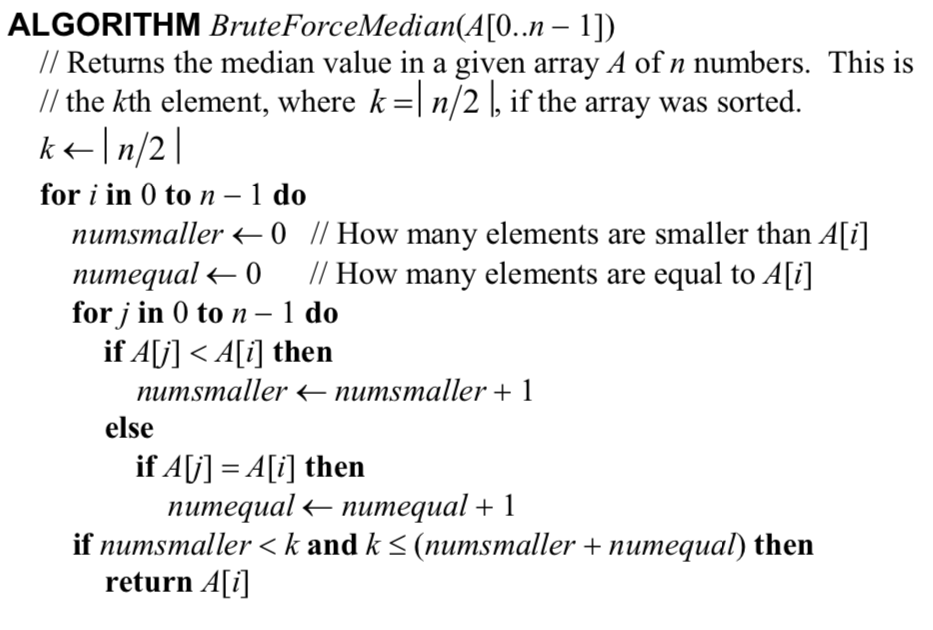
\includegraphics[width=0.7\linewidth]{Results/AlgorithmPseudocode}
	\caption{The pseudocode for the BruteForceMedian algorithm.}
	\label{fig:algorithmpseudocode}
\end{figure}

	
	\subsection{Average case:}
	In comparison to other methods of finding the median, this algorithm is not efficient due to checking all elements of the array with eachother. The \textit{\textbf{BruteForceMedian}} has a theoretical computational efficiency on the order of $\Theta(n^2)$. We can prove this theoretically by doing the following.
	
	The average case efficiency of the algorithm can be theoretically determined by considering the number of operations required to determine the median. Consider the array of size $n$, such that $A = [a_1,a_2,a_3,...a_n]$, where the median value of the array will be placed at the $kth$ position. To determine the median of this array, the algorithm will need to check every element in the array including itself. As a result, the algorithm must performed $nktimes n$ of comparison for the median to be $A[k]$. If we assume that the median has an equal chance of being at any position in the array, then the average number of operations to determine the median will be number of operations over the length of the array (or in other words half the length of the array). The definition we have arrived at is the statistical true median (half of the set of observations), as defined by \textit{WolframMathWorld} \cite{RN4}. This can be expressed as, $(k=A[j])\forall_j\in[0,1,2,3,...n-1]$ where k is the median, and A is the array. Therefore, the average case will be the iteration through all elements of the array, over the length of the array.
	
	\begin{align*}
	 C_{average} &= \sum\limits_{j=1}^{n}\frac{j \times n}{n} \\
	 					&= \sum\limits_{j=1}^{n}j\\
	 					&= \frac{n(n+1)}{2}\\
	 					&\approx\frac{1}{2}n^2\\
	 					\therefore C_{average} &\in \Theta(n^2)
	\end{align*}
	
	When there is an even number of elements, the algorithm always chooses the element to the left of the midpoint of the array. In this sense, the find the true number of elements, we must consider the partity between both even and odd arrays. Consider the two arrays $A_{even} = [a_1,a_2,a_3,...a_n]$ and $B_{odd} = [b_1,b_2,b_3,...b_{n+1}]$. The average number of comparisons between each of these arrays is going to be dependant on iterating through each of these arrays for all elements in the array. If we take the average case from broth arrays, we get.
	
	\begin{align*}
		C_{odd} &= \frac{n^2+n}{2}\\
		C_{Even} &= \frac{n^2}{2}
	\end{align*}

	In this sense, the odd case has one more iteration through the length of the array compared with the even array. This can be attributed to the definition we defined previously, whereby $A_{even} = [a_1,a_2,a_3,...a_n]$ and $B_{odd} = [b_1,b_2,b_3,...b_{n+1}]$. We can combine these two equations to get the overall average. Note that the even will be modulo 2 because even numbers are divisible by 2.
	
	\begin{align*}
C_{average} &= \frac{n^2+(n\mod 2)n}{2}
	\end{align*}

	\subsection{Best case:}
	The best case of the algorithm will be if the median is the first element in the array, therefore the algorithm will only have to check all the elements in the array once. In this case, the algorithm does not past the first iteration of the outer for loop. 
	Consider the situation in which you have the array $A=[k,a_2,a_3,...,a_n]$ where the first element in the array is the median $k$. In this case, the algorithm only iterates over the whole array to find out the number of smaller and equal comparisons. This can be simply put as,
	
	\begin{align*}
	C_{best} &= \sum\limits_{i=1}^{n}1\\
				&= n-1+1\\
				&= n\\
				\therefore C_{best} &\in \Theta(n)
	\end{align*}
	
	
	\subsection{Worst case:}
	The worst case of the algorithm is that if the median is in the last element in the array. In this situation, the algorithm will have to go through all possible iterations of comparisons. Consider the situation in which we have an array of $A=[a_1,a_2,a_3,...a_n]$. In the worst case situation, we can assume that $a_n$ will be the median. The worst case can then be expressed as the comparison of all elements up to the last element $a_n$.
	
	\begin{align*}
	C_{worst} &= \sum\limits_{i=1}^{n} \sum\limits_{j=1}^{n}2\\
					&= (n-1+1)(n-1+1)2\\
					&= 2n^2\\
	\therefore C_{worst} &\in \Theta(n^2)
	\end{align*}
	
	
\section{Methodology, Tools and Techniques}
	\subsection{Programming environment}
	The testing, computation, execution and compilation of the program was completed on a 2018 15” Macbook Pro running macOs Mojave (10.14.2). This computer has a 2.2GHz Intel core i7 (6 core) processor, 16 GB 2400 MHz DDR4 RAM and a Radeon Pro 555X GPU. Compilation was performed using the Clang++17 compiler in accordance to the ISO/IEC 14882:2017 current standard and execution was performed on JetBrains CLion Interactive Development Environment (version 2019.1) using cmake (version 3.11).
	\subsection{Programming language implementation}
	The decision to implement the algorithm in C++ as opposed to C\# or Java came down to speed, current development environment and personal reasons. C++ is quite similar to C as in it is very lightweight and has manual memory management. For analysis of algorithms, it is important that compilation time is low, and that memory management is efficient. In addition to the above, the development environment was within the macOS operating system. C\# is targeted towards windows developers, and hence has more support. Further to the above, I believed that this was a good opportunity to learn C++, following on from my experience in C.
	\subsection{Implementation of program}
	The initial requirements stated that the algorithm should be implemented in the most faithful way, and a selection of tests would be made to confirm the functionality, operational and time efficiencies of the algorithm. It was then proposed that the user would be able to control the variables for each of the tests from the command line. In addition to this, the program would be able to produce each of the test input arrays automatically from the user inputs, feed this through the \textit{\textbf{BruteForceMedian}} algorithm, and then store the input and output arrays as a csv for analysis as well as print the tests to the console. From start to finish, this is the process the user would take to execute the program. 
	\begin{enumerate}
		\item The user will navigate to the \textit{headerFile.h} to input the variables for each of the tests (the variables are stored as pre-processor directives to limit the variables in the global scope of the program). These variables and their definitions can be found in the appendix at table \ref{tab:preprocessordirectives}.
		\item The user will compile and run the program. The program will run and display the current variables it is using for the test to the console.
		\item The user will be prompted to enter the test they would like to complete (0 = FUNCT\newline-IONALITY, 1 = OPERATIONAL, 0 = TIMING)
		\item The user will enter the test they would like to perform, and the program will print each of the tests and the results to the console. In addition to this, the program will save all test input and output data to csv files (in the same location as the executable file).
	\end{enumerate}
	For a more detailed top down diagram of the program as a whole, functions used within each file, linkages between files, and the preprocessor directives, see the appendix table \ref{tab:preprocessordirectives} and figure \ref{fig:programoverview}. 
	
	The experimental data used in the analysis of the algorithm was obtained by running the program with the input variables (as specified in the method above). Post analysis regarding graphs, regression analysis and finding the average, worst and best-case efficiencies was done using Microsoft Excel. 

	\subsection{Implementation of algorithm}
	The algorithm was implemented in two separate files to separate the timing tests and the operational tests:
\begin{itemize}
	\item[-]\textit{“algorithmOps.cpp”} $\rightarrow$ File which stores the implementation for the number of operations in the algorithm.
	\item[-]\textit{“algorithmTime.cpp”} $\rightarrow$ File which stores the implementation for the computational time of the algorithm.
\end{itemize}
	Between the two files, the only difference was that the operational implementation included a global variable to track the operational count, whereas the timing file did not include this variable. For the purpose of being succinct, the operational implementation in the \textit{“algorithmOps.cpp”} file will be discussed. 
	
	The algorithm inputs a pointer to a vector of ints and returns the median as an int. If the array has a length of 0, the function returns 0 (this is the error condition where the input array has not length). The basic operations of the algorithm is stored in a global variable named \textit{numOps}. The computation time of the algorithm was measured by using a \textit{high\_resolution\_clock} in the std namespace and calling the algorithm implementation in the \textit{“algorithmTime.cpp”} file. The data types where decided based on the theoretical size required for each of the variables. As the tests are not exceeding anything above the limitation for ints in C++ (4bytes -2147483647 to 2147483647), ints were used for all of the variables (with the exception to the number of operations which was a \textit{unsigned long long int}). Please refer to listing \ref{lst:BruteForceMedianOps} for the \textit{“algorithmOps.cpp”} file.
	
	\begin{lstlisting}[caption={BruteForceMedian algorithm implementation - \textit{algorithmOps.cpp} (operations implementation)}, label={lst:BruteForceMedianOps}, language=C++]  
	unsigned long long numOp = 0;
	
	int BruteForceMedian(vector<int> &A)
	{
		int size = A.size(); // Calculating the size fo the input array
		int k = (int) ceil(A.size() / 2.0); // Calculate half array.
		
		for (int i = 0; i <= (size-1); i++) {
			int numSmaller = 0; // Number of elements smaller than A[i];
			int numEqual = 0; // Number of elements equal to A[i];
			
			for (int j = 0; j <= (size-1); j++) {
				if (A[j] < A[i]) {
					numSmaller+=1;
					numOp+=1;
				} else {
					if (A[j] == A[i]) {
						numEqual+=1;
						numOp+=1;
					}
				}
			}
			if ((numSmaller < k) && (k <= (numSmaller + numEqual))) {
				return A[i];
			}
		}
		return 0;
	}
	\end{lstlisting}
	
\section{Experimental design}
The design of the experiments is broken down into three different subsections. Below is a succinct summary of each of the three tests (table \ref{tab:testtype}).

\begin{table}[H]
	\centering
	\caption{Types of tests performed}
	\label{tab:testtype}
	\resizebox{\textwidth}{!}{%
		\begin{tabular}{lL{0.65\textwidth}lL{0.65\textwidth}l}
			\hline
			Test Name & Purpose &  \\ \hline
			Functional test & To test the functionality of the program and the algorithm. This will confirm that the program and the algorithm are working as intended. &  \\ \cline{1-2}
			Operational test & Testing the operational efficiency of the algorithm. This test relates to the number of operations performed within the algorithm, and the efficiency class of the algorithm. &  \\ \hline
			Timing test & To test the time complexity of the algorithm. This test calculates the execution time of the algorithm for a given array size. &  \\ \cline{1-2}
		\end{tabular}
	}
\end{table}
For each of the above tests, there are subtests which are performed. These subtests have been designed to validate the purpose of the test class. 

\subsection{Functional tests (methodology):}
To ensure the functional correctness off the algorithm and the program, a number of subtests have been created. The subtests which have been created assess the extreme (boundary) conditions of the algorithm, and to ensure functionality. The tests are as follows:
\begin{itemize}
	\item[-]Negative array elements
	\item[-]Odd length of array
	\item[-]Even length of array
	\item[-]Large length of array	
	\item[-]One length array
	\item[-]No length array
	\item[-]Random array size and elements
	\item[-]Random array size and reversed sorted elements
	\item[-]Random array size and sorted elements
\end{itemize}
To ensure that the test has passed, the brute force median result is compared another median finding algorithm (comparison algorithm). The comparison algorithm is stored in the \textit{“comparison-Algorithm.cpp”} (refer to the appendix listing \ref{lst:comparison}). This algorithm takes in a vector of ints and returns the median as an int.  The general premise of this algorithm is to sort the input vector in ascending order using the sorting method from the standard c++17 library. After this vector has been sorted, it will be check to see if it is an even length or an odd length vector. If it is an even length vector, we return the ceiling function of the difference of the elements which are indexed at half of the length of the vector and half of the length of the vector minus one. If the input vector is  an odd length vector, we return the element which is half the length if the input vector. This is an adaptation of an algorithm which has been proven to be correct by the community on \textit{stackoverflow.com} as well as \textit{geeksforgeeks.com}\cite{RN2} \cite{RN3}. This algorithm has a a run time complexity of $\Theta (n\log(n))$ due to the sorting at the beginning of the algorithm.

If the median between the \textbf{\textit{BruteForceMedian}} implementation algorithm and the \textbf{\textit{Comparison-Algorithm}} are the same, then the test will pass. Throughout all of the tests below, the output data is stored as an integer in a 2-dimensional array of vectors (in C++ vectors are a resizable arrays). The implementation for each of the subtests can be found in the appendix under test algorithms. 

\subsubsection{Negative elements (NEGATIVE): }
In general, the negative arrays are produced as a set of 2 dimensional vectors, whereby the inner vector is an array of negative elements from 0 to the simulation size, and the outer vector is the collection of negative arrays. The size of the negative array is dependent on the number of simulations which the user inputs. 
\subsubsection{Odd length (ODD): }
The odd length arrays are generated by iterating through 0 to the amount of simulations, as specified by the user, in odd steps. This is stored in an inner vector, which is then stored in an outer vector (the outer vector being the collection of inner vectors). 
\subsubsection{Even length (EVEN): }
The even length arrays are generated in the same way as the odd length, however the step size for this array collection is even instead of odd. 
\subsubsection{Large array length (LARGE): }
The large arrays are generated based on the input from the user (as in the user can specify the length of the large array). In addition to this, the user can specify the number of simulations to be run on that array length that they specified. 
\subsubsection{One length (ONELEN): }
This test is produced by creating a vector with a length of 1. The elements inside the vector are positive integers with a value of 1. The purpose of this test is to confirm the functionality of the algorithm and the program with a input vector of 1.

\subsubsection{No length (NOLEN): }
The purpose of this test is to confirm the functionality of the error return path of the algorithm. In this case, the algorithm has an error path which returns 0 for an input array of length 0. If the input vector is 0, then the expected result for this test case will be 0. This is also compared to the median value (as calculated by the \textbf{\textit{ComparisonAlgorithm}}), which will have a value of 0, because there are no elements in the array. In this case, if the output value is 0, then the test will pass.

\subsubsection{Random array size of random elements (RANDOM): }
This test is to confirm the functionality of the algorithm over a random of random input length and elements. Each of the elements in the input array are randomly generated using a seed. The location of each of the elements in the array is unique, and no two elements are the same in the array (detailed explanation of the generation of this test can be found in the operational testing and timing testing (methodology) section).

\subsubsection{Random array size of reversed sorted elements (REVERSED): }
The input array for this test were filled with reversed sorted consecutive integers, up to the length of the array. The purpose of this test was to assess the functionality of the algorithm under a sorted condition (detailed explanation of the generation of this test can be found in the operational testing and timing testing (methodology) section).

\subsubsection{Random array size of sorted elements (SORTED): }
This test was to confirm the functionality of the algorithm under a sorted condition. It is different from the reversed sorted elements test above because the elements are consecutive, sorted and in the right order (detailed explanation of the generation of this test can be found in the operational testing and timing testing (methodology) section).

\subsection{Operational testing and timing testing (methodology):}
For each of the operational and timing tests, there are a number of the same subtests performed. These subtests are to assess the performance of the algorithm, rather than the functionality. In this sense, the tests are based on the elements of the array, rather than the boundary conditions of the input to the algorithm. The subtests are as follows:
\begin{itemize}
	\item[-]Random array size and elements
	\item[-]Random array size and reversed sorted elements
	\item[-]Random array size and sorted elements
\end{itemize}

The process for obtaining the input data for each of the tests above is somewhat similar to the functional test. The data is stored as an integer, within a 2-dimensional re-sizable array. The user can specify the step size between each random size array, the number of simulations performed for the array with the same length, the range of the random variable generated and the number of simulations. The random value is generated using a seed based on the current clock time of the computer (found in \textit{“generateData.cpp”}). The range is specified by taking the modulo of the random number generated by the maximum number in the range (defined by \textit{RANDOM\_RANGE} in the \textit{“headerFile.h”}). The program creates multiple of the same length array (as defined by \textit{ARRAY\_NUM\_SIMS}) to find the average, best and worst-case efficiencies for a certain array length. In addition to this, the length of the array is stepped based on the \textit{ARRAY\_STEP\_SIZE} variable. The amount of simulations (defined by \textit{SIMULATIONS}) is the amount of the same length array. For example, if the user selected the following variables, \textit{ARRAY\_NUM\_SIMS} = 10, \textit{ARRAY\_STEP\_SIZE} = 100 and \textit{SIMULATIONS} = 10, then they would get an input 2-dimensional array of 10 sets of 10 arrays with the same length, with their length stepped by 100 up to a length of 1000.

The best, worst and average case efficiencies for both the operational testing and the timing testing was considered. The methodology to obtain these results consisted of taking the average across the number of the same simulation sized arrays, the maximum value and the minimum value. In this case, the average value was considered as the average case of the algorithm, the maximum value was the worst case, and the minimum value was the best case. This was then plotted against the size of the array for the given execution time and operation count. In addition to the above method, the regression tool in excel was also used to gather the $r^2$ value and the line of best fit. This was then recorded in a table, which can be found in the appendix section of this report. 

\subsection{Operational testing (numOps location):}
The main point of interest for the operational testing is where the number of operations are counted for in the algorithm. As defined in the implementation of the algorithm section, the number of operations is stored in a global variable of type \textit{unsigned long long} named \textit{numOp} in the file \textit{“algorithmOps.cpp”}. This variable is then incremented when the algorithm performs an “operation”. Operation is defined as a comparison between two elements within the input array, or an increment of a variable in the local scope of the function. This occurs when the \textit{numSmaller} and \textit{numEqual} variables are incremented. In addition, this is when a comparison is made between two elements in the input array (please refer to the appendix listing \ref{lst:bruteforceops}).
\subsection{Timing testing (time measurement location):}
The time was kept separate from the operational testing implementation. As a result, the time was measured using the \textbf{\textit{BruteForceMedianTime}} function in the \textit{“algorithmTime.cpp”} file. The time was measured before and after this function was called in the \textit{“runTests.cpp”} file. The C++17 \textit{high\_resolution\_clock} was used to measure the time, in nanoseconds, points before and after the function call. The difference was taken between these two points, and then added to a vector, \textit{execTimeVector} which stores the execution time for each test, for later use in the program. 

\section{Experimental results}
This section will explain the purpose of each test, discuss the input variables, display the results from each of the tests, interpret the results in the context of the test, analyse the results compared to theoretical assumptions, and explain any discrepancies in the data. 

\subsection{Functional tests:}
The results for the functional tests are broken down into tables, where the median result from the \textbf{\textit{BruteForceAlgorithm}} is compared with the result from the \textbf{\textit{ComparisonAlgorithm}}. If these two match, the then test passes, whereas if they don't match, then the test does not pass. In addition to the above, the input variables for the functional test have been detailed in the appendix under test results, and also below in table \ref{tab:subtestvariables}.


\begin{table}[H]
	\centering
	\caption{These are the variables which are being used for all subtests under the functional test.}
	\label{tab:subtestvariables}
	\resizebox{\textwidth}{!}{%
		\begin{tabular}{lL{0.65\textwidth}l}
			\textbf{Variable} & \textbf{Value} \\ \hline
			LARGE\_ARRAY\_VALUE & 20000 \\ \hline
			LARGE\_ARRAY\_SIMS & 1 \\ \hline
			ARRAY\_STEP\_SIZE & 501 \\ \hline
			ARRAY\_NUM\_SIMS & 250 \\ \hline
			RANDOM\_RANGE & 10000 \\ \hline
			SIMULATIONS & 10 \\ \hline
		\end{tabular}%
	}
\end{table}

\subsubsection{Negative array elements (NEGATIVE): }
In this test, we used an array length of size 11, with all elements of the array being negative consecutive elements. The point of this test was to test the functionality of the algorithm with negative numbers. As it can be seen, all tests passed.
\begin{table}[H]
	\centering
	\caption{Negative array elements test results.}
	\label{my-label}
	\resizebox{\textwidth}{!}{%
		\begin{tabular}{lllll}
			\textbf{TestNumber} & \textbf{InputArrayLength} & \textbf{AlgoMedianValue} & \textbf{CalculatedMedianValue} & \textbf{PASS/FAIL} \\ \hline
			0 & 11 & -5 & -5 & PASS \\ \hline
			1 & 11 & -5 & -5 & PASS \\ \hline
			2 & 11 & -5 & -5 & PASS \\ \hline
			3 & 11 & -5 & -5 & PASS \\ \hline
			4 & 11 & -5 & -5 & PASS \\ \hline
			5 & 11 & -5 & -5 & PASS \\ \hline
			6 & 11 & -5 & -5 & PASS \\ \hline
			7 & 11 & -5 & -5 & PASS \\ \hline
			8 & 11 & -5 & -5 & PASS \\ \hline
			9 & 11 & -5 & -5 & PASS
		\end{tabular}%
	}
\end{table}

\subsubsection{Odd length of array (ODD): }
The purpose of this test is to confirm the functionality of the algorithm for an odd length array. The test uses consecutive odd length arrays up to 19, filled with consecutive sorted positive integers.
\begin{table}[H]
	\centering
	\caption{Odd length of array elements test results.}
	\label{my-label}
	\resizebox{\textwidth}{!}{%
		\begin{tabular}{lllll}
			\textbf{TestNumber} & \textbf{InputArrayLength} & \textbf{AlgoMedianValue} & \textbf{CalculatedMedianValue} & \textbf{PASS/FAIL} \\ \hline
			0 & 1 & 1 & 1 & PASS \\ \hline
			1 & 3 & 2 & 2 & PASS \\ \hline
			2 & 5 & 3 & 3 & PASS \\ \hline
			3 & 7 & 4 & 4 & PASS \\ \hline
			4 & 9 & 5 & 5 & PASS \\ \hline
			5 & 11 & 6 & 6 & PASS \\ \hline
			6 & 13 & 7 & 7 & PASS \\ \hline
			7 & 15 & 8 & 8 & PASS \\ \hline
			8 & 17 & 9 & 9 & PASS \\ \hline
			9 & 19 & 10 & 10 & PASS
		\end{tabular}%
	}
\end{table}

\subsubsection{Even length of array (EVEN):}
This test consisted of consecutive even length arrays up to a  length of 18 filled with consecutive sorted positive integers. The purpose of this test was to confirm the functionality of the algorithm under an even length array. It can be seen that these tests failed.
\begin{table}[H]
	\centering
	\caption{Even length of array elements test results.}
	\label{tab:even}
	\resizebox{\textwidth}{!}{%
		\begin{tabular}{lllll}
			\textbf{TestNumber} & \textbf{InputArrayLength} & \textbf{AlgoMedianValue} & \textbf{CalculatedMedianValue} & \textbf{PASS/FAIL} \\ \hline
			0 & 0 & 0 & 0 & PASS \\ \hline
			1 & 2 & 1 & 2 & FAIL \\ \hline
			2 & 4 & 2 & 3 & FAIL \\ \hline
			3 & 6 & 3 & 4 & FAIL \\ \hline
			4 & 8 & 4 & 5 & FAIL \\ \hline
			5 & 10 & 5 & 6 & FAIL \\ \hline
			6 & 12 & 6 & 7 & FAIL \\ \hline
			7 & 14 & 7 & 8 & FAIL \\ \hline
			8 & 16 & 8 & 9 & FAIL \\ \hline
			9 & 18 & 9 & 10 & FAIL
		\end{tabular}%
	}
\end{table}

\subsubsection{Large length of array (LARGE): }
The large array of elements test used the \textit{LARGE\_ARRAY\_VALUE} and the \textit{LARGE\_ARRAY\_SIMS} variables as specified by the user to create the input array data. In this case, the test was setup that it would test an array with a length of 20000, filled with consecutive sorted integers up to 20000. In this case, the test passed.
\begin{table}[H]
	\centering
	\caption{Large length of array elements test results.}
	\label{my-label}
	\resizebox{\textwidth}{!}{%
		\begin{tabular}{lllll}
			\textbf{TestNumber} & \textbf{InputArrayLength} & \textbf{AlgoMedianValue} & \textbf{CalculatedMedianValue} & \textbf{PASS/FAIL} \\ \hline
			0 & 19999 & 10000 & 10000 & PASS \\ \hline
		\end{tabular}%
	}
\end{table}

\subsubsection{One length array (ONELEN):}
This test was completed to assess the functionality of the algorithm regarding an array of one length. Ten tests were completed of the same array, and all elements in the array were of an integer value of 1 (with the exception of the first array which was filled with an integer value of 0). All of the tests passed.

\begin{table}[H]
	\centering
	\caption{One length of array elements test results.}
	\label{my-label}
	\resizebox{\textwidth}{!}{%
		\begin{tabular}{lllll}
			\textbf{TestNumber} & \textbf{InputArrayLength} & \textbf{AlgoMedianValue} & \textbf{CalculatedMedianValue} & \textbf{PASS/FAIL} \\ \hline
			0 & 1 & 0 & 0 & PASS \\ \hline
			1 & 1 & 1 & 1 & PASS \\ \hline
			2 & 1 & 1 & 1 & PASS \\ \hline
			3 & 1 & 1 & 1 & PASS \\ \hline
			4 & 1 & 1 & 1 & PASS \\ \hline
			5 & 1 & 1 & 1 & PASS \\ \hline
			6 & 1 & 1 & 1 & PASS \\ \hline
			7 & 1 & 1 & 1 & PASS \\ \hline
			8 & 1 & 1 & 1 & PASS \\ \hline
			9 & 1 & 1 & 1 & PASS
		\end{tabular}%
	}
\end{table}

\subsubsection{No length array (NOLEN): }
The test below was to confirm the functionality of the program as well as the algorithm itself. All of the tests passed.
\begin{table}[H]
	\centering
	\caption{No length of array elements test results.}
	\label{my-label}
	\resizebox{\textwidth}{!}{%
		\begin{tabular}{lllll}
			\textbf{TestNumber} & \textbf{InputArrayLength} & \textbf{AlgoMedianValue} & \textbf{CalculatedMedianValue} & \textbf{PASS/FAIL} \\ \hline
			0 & 0 & 0 & 0 & PASS \\ \hline
			1 & 0 & 0 & 0 & PASS \\ \hline
			2 & 0 & 0 & 0 & PASS \\ \hline
			3 & 0 & 0 & 0 & PASS \\ \hline
			4 & 0 & 0 & 0 & PASS \\ \hline
			5 & 0 & 0 & 0 & PASS \\ \hline
			6 & 0 & 0 & 0 & PASS \\ \hline
			7 & 0 & 0 & 0 & PASS \\ \hline
			8 & 0 & 0 & 0 & PASS \\ \hline
			9 & 0 & 0 & 0 & PASS
		\end{tabular}%
	}
\end{table}

\subsubsection{Random array size of elements (RANDOM): }
This test is to confirm the functionality of the algorithm, in that it is calculating the correct mean for a range of different input lengths and input values. The input array is an array from length 11 to 110, with step sizes of 10. The random numbers in the input array were generated using a random seed from the current clock time of the computer. It can be seen that the tests pass on odd length arrays, but fail on even length arrays. The input arrays will not be displayed in the appendix for neatness sake. 
\begin{table}[H]
	\centering
	\caption{Random array size and elements}
	\label{my-label}
	\resizebox{\textwidth}{!}{%
		\begin{tabular}{lllll}
			\textbf{TestNumber} & \textbf{InputArrayLength} & \textbf{AlgoMedianValue} & \textbf{CalculatedMedianValue} & \textbf{PASS/FAIL} \\ \hline
			0                   & 11                        & 36001                    & 36001                          & PASS               \\ \hline
			1                   & 22                        & 42383                    & 44166                          & FAIL               \\ \hline
			2                   & 33                        & 68724                    & 68724                          & PASS               \\  \hline
			3                   & 44                        & 48053                    & 50016                          & FAIL               \\  \hline
			4                   & 55                        & 58736                    & 58736                          & PASS               \\ \hline
			5                   & 66                        & 40751                    & 42081                          & FAIL               \\ \hline
			6                   & 77                        & 46016                    & 46016                          & PASS               \\ \hline
			7                   & 88                        & 55440                    & 55810                          & FAIL               \\ \hline
			8                   & 99                        & 49922                    & 49922                          & PASS               \\ \hline
			9                   & 110                       & 49759                    & 49986                          & FAIL              
		\end{tabular}%
	}
\end{table}

\subsubsection{Random array size of reversed sorted elements (REVERSED): }
The input array for this test were filled with reversed sorted consecutive integers, up to the length of the array. Each of the array sizes were randomized from 11 to 121 with a step size of 10. The purpose of this test was to assess the functionality of the algorithm under a sorted condition. All of the odd tests passed, whereas all of the even tests failed. 
\begin{table}[H]
	\centering
	\caption{Random array size with reversed consecutive sorted elements}
	\label{my-label}
	\resizebox{\textwidth}{!}{%
		\begin{tabular}{lllll}
			\textbf{TestNumber} & \textbf{InputArrayLength} & \textbf{AlgoMedianValue} & \textbf{CalculatedMedianValue} & \textbf{PASS/FAIL} \\
			0                   & 11                        & 5                        & 5                              & PASS               \\ \hline
			1                   & 22                        & 10                       & 11                             & FAIL               \\ \hline
			2                   & 33                        & 16                       & 16                             & PASS               \\ \hline
			3                   & 44                        & 21                       & 22                             & FAIL               \\ \hline
			4                   & 55                        & 27                       & 27                             & PASS               \\ \hline
			5                   & 66                        & 32                       & 33                             & FAIL               \\ \hline
			6                   & 77                        & 38                       & 38                             & PASS               \\ \hline
			7                   & 88                        & 43                       & 44                             & FAIL               \\ \hline
			8                   & 99                        & 49                       & 49                             & PASS               \\ \hline
			9                   & 110                       & 54                       & 55                             & FAIL               \\ \hline
			10                  & 121                       & 60                       & 60                             & PASS              
		\end{tabular}%
	}
\end{table}



\subsubsection{Random array size of sorted elements (SORTED): }
This test was to confirm the functionality of the algorithm under a sorted condition. It is different from the reversed sorted elements test above because the elements are consecutive, sorted and in the right order. Each of the input array lengths have been randomized from 11 to 121 with a step size of 10. The results displayed that the even tests have failed, whereas the odd tests have passed.

\begin{table}[H]
	\centering
	\caption{Random array size with sorted consecutive elements}
	\label{my-label}
	\resizebox{\textwidth}{!}{%
		\begin{tabular}{lllll}
			\textbf{TestNumber} & \textbf{InputArrayLength} & \textbf{AlgoMedianValue} & \textbf{CalculatedMedianValue} & \textbf{PASS/FAIL} \\
			0                   & 11                        & 5                        & 5                              & PASS               \\ \hline
			1                   & 22                        & 10                       & 11                             & FAIL               \\ \hline
			2                   & 33                        & 16                       & 16                             & PASS               \\ \hline
			3                   & 44                        & 21                       & 22                             & FAIL               \\ \hline
			4                   & 55                        & 27                       & 27                             & PASS               \\ \hline
			5                   & 66                        & 32                       & 33                             & FAIL               \\ \hline
			6                   & 77                        & 38                       & 38                             & PASS               \\ \hline
			7                   & 88                        & 43                       & 44                             & FAIL               \\ \hline
			8                   & 99                        & 49                       & 49                             & PASS               \\ \hline
			9                   & 110                       & 54                       & 55                             & FAIL               \\ \hline
			10                  & 121                       & 60                       & 60                             & PASS              
		\end{tabular}%
	}
\end{table}

\subsection{Operational test}
The purpose of the operational tests is to confirm the number of operations the algorithm perform for a given array input size. The results below are split into graphs (which display the average, worst and best cases for each test) and a regression analysis (which displays the line of best fit, and the $r^2$ which is a measure of deviance from the line of best fit). The regression results can be found in the appendix, whereas the graphs can be found under this section. All results displayed a strong quadratic trend, which is in line with the theoretical expectations. For neatness sake, all of the graphs for this section are shown in the appendix under operational test.

\subsection{Timing test}
The purpose of the timing test was to assess the time efficiency of the algorithm for a given input size. The results below display the data for the average, worst and best cases. In addition to that a line of best fit has been plotted against the data from the regression analysis (details of the regression analysis can be found in the appendix). The results show a strong quadratic trend for all the average and worst case, which is in line with theoretical expectations. In addition to this, the random array size of random elements has a best case which is linear, which is what we expect from the theoretical calculations. A detailed analysis will be completed in the analysis section of this report. For neatness sake, all of the graphs for this section are shown in the appendix under timing test.

\section {Experimental analysis:}
\subsection{Functional tests}
All of the functional tests passed with the exception of the even array length test (refer to table \ref{tab:even}). In addition, the random length array tests failed for arrays which had an even length.  This was to be expected, because it was theoretically proven that the algorithm selects the left of the midpoint when there is an even array. This is support to suggest that the algorithm does not take the true median of the array. In effect, this is a limitation to the algorithm, which can be improved by using other algorithms discussed in the recommendations section of this report.  

\subsection{Operational test}
\begin{figure}[H]
	\centering
	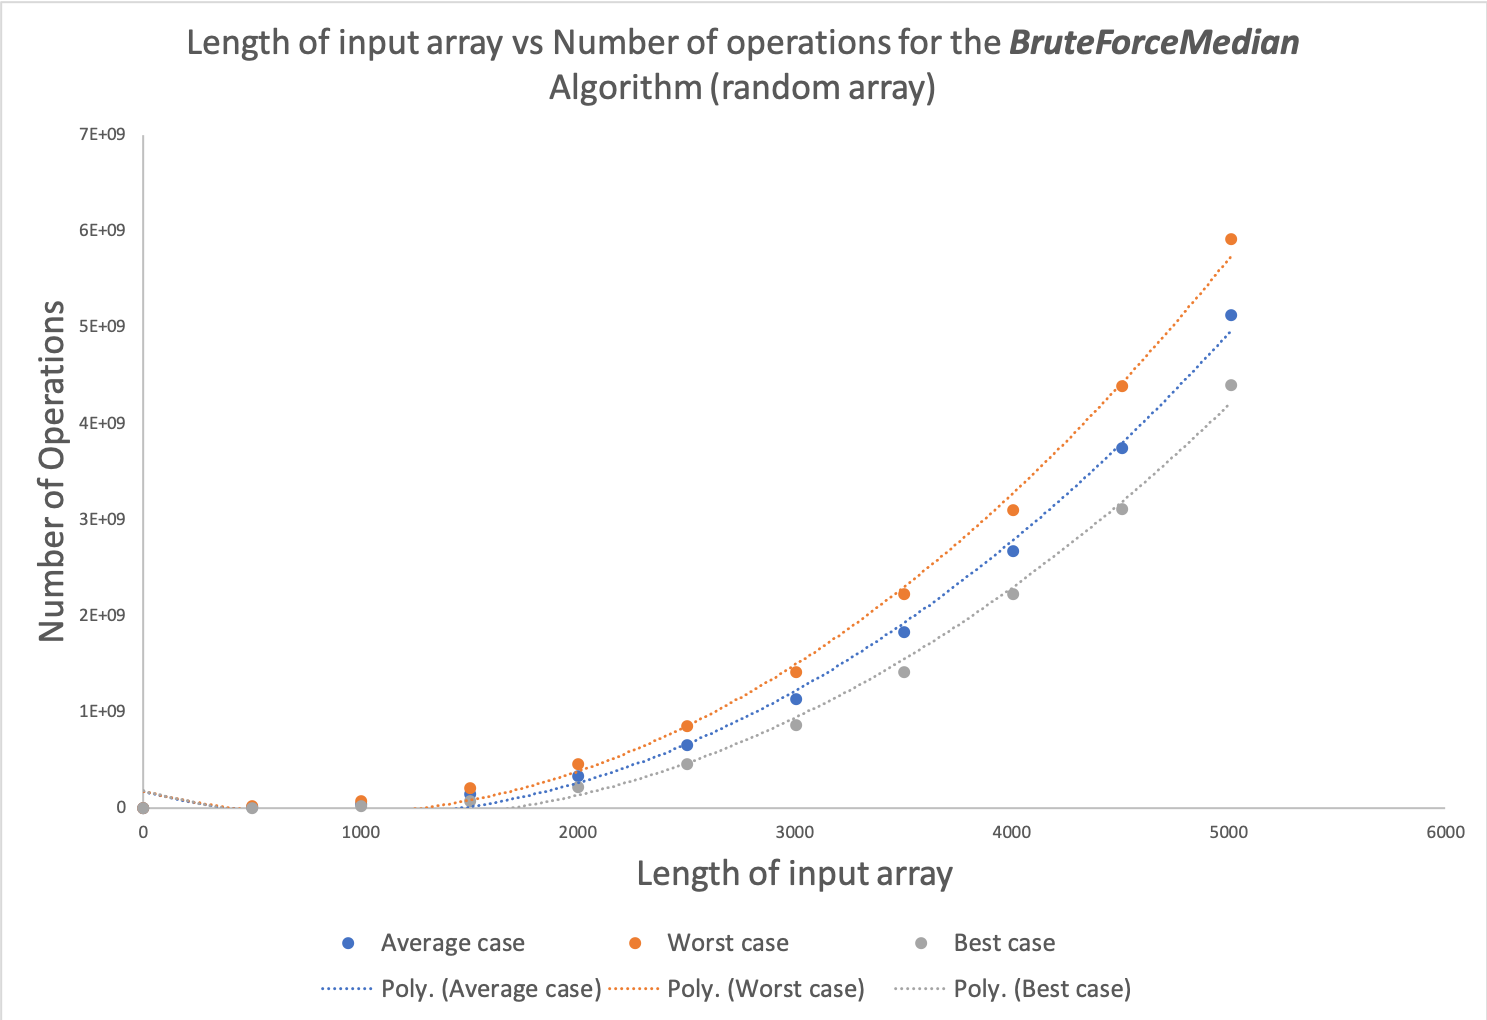
\includegraphics[width=0.75\linewidth]{Results/OpsRandom}
	\caption{Random array size of random elements vs the operational count.}
	\label{fig:opsrandomAnalysis}
\end{figure}

The operational test results were inline with the theoretical efficiency of $\Theta (n^2)$. Each of the test cases can be seen to have a strong quadratic trend (refer to the operational test section of the appendix, specifically figures \ref{fig:opsrandom}, \ref{fig:opsreversed} and \ref{fig:opssorted}). This is supported by the regression analysis performed after the results were obtained (refer to the appendix section test results, regression analysis table \ref{tab:randomOps},\ref{tab:reversedOps} and \ref{tab:sortedOps}). The average case represented a strong quadratic trend, as can be seen in the random graph above (figure \ref{fig:opsrandomAnalysis}). In addition to this, the range between the worst and best cases was quite narrow. This suggests that the variance in the random numbers does not effect the number of operations performed by the algorithm. From theoretical analysis, this would seem to be correct, as the algorithm has to perform the number of comparisons no matter if the median is the first element in the array or the last element in the array. For example, the best case for the number of operations would be that the median is the first element in the array. In any case, the algorithm still has to compute the number of basic operations as the length of the array, multiplied by each element. This equates to the theoretical efficiency of $\Theta (n^2)$, and is supported in the empirical analysis. 
What appeared to be interesting is that the reverse sorted and sorted element tests seemed to have a higher number of operations compared to the random element test. This would seem to be the case, as the random elements could have had the median closer to the front end of the array, and as a result less operations would be performed. This is in comparison to the sorted tests, whereby the algorithm would have to go through each element in the array, until it found the median (which in the sorted case the median would always be at half the length of the array).

\subsection{Timing test}
\begin{figure}[H]
	\centering
	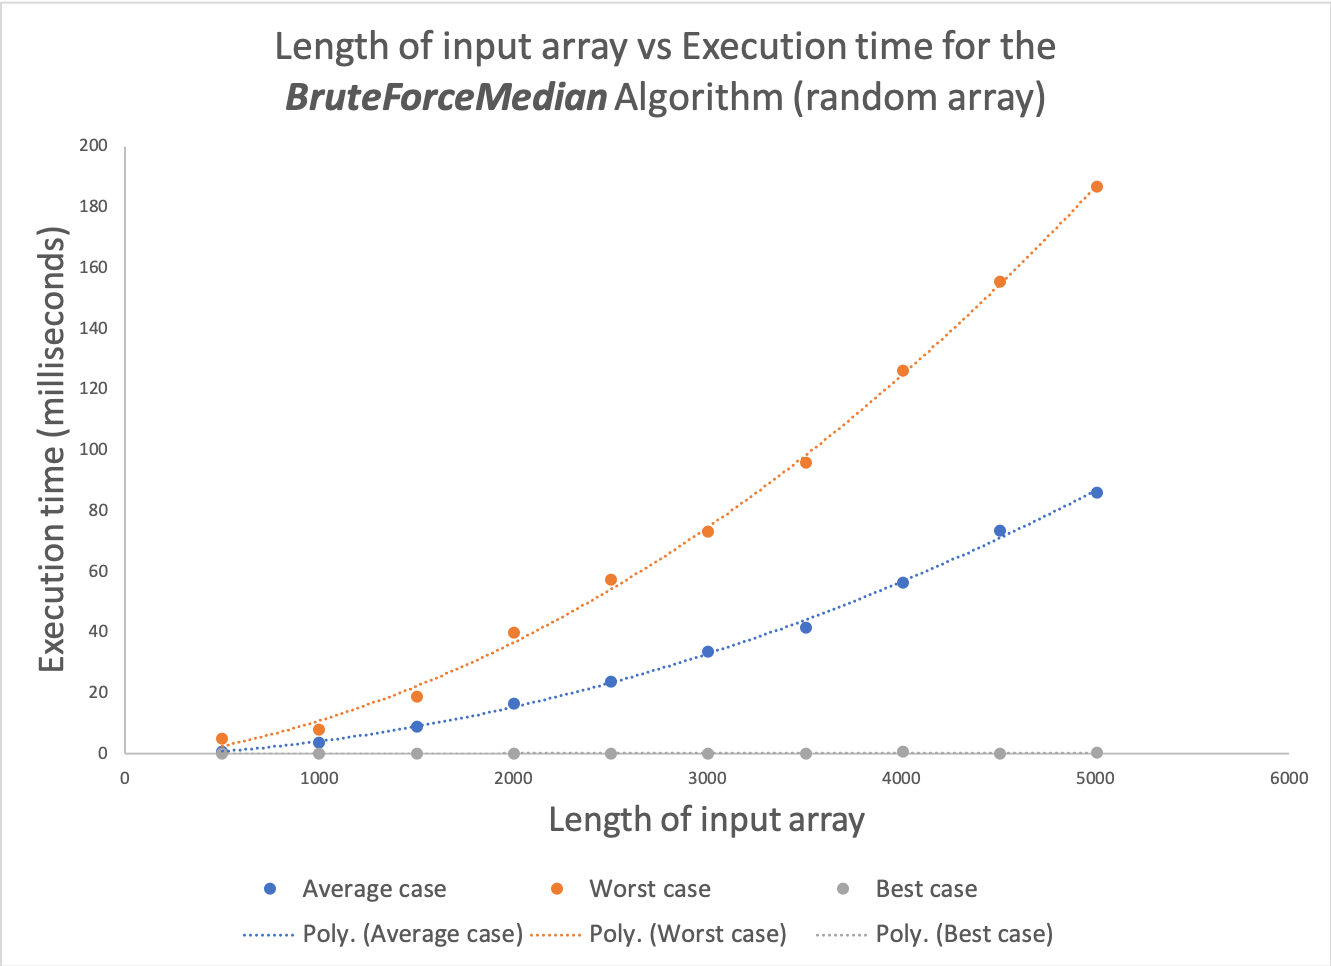
\includegraphics[width=0.75\linewidth]{Results/TimeRandom}
	\caption{Random array size of random elements vs the execution time of each test.}
	\label{fig:timerandomAnalysis}
\end{figure}

The timing test results supported the theoretical average efficiency of the algorithm of $\Theta (n^2)$. Most notably, the random array size of random element test results displayed a relationship which was identical to the theoretical efficiency for the average, worst and best cases of the algorithm (Figure \ref{fig:timerandomAnalysis}). The regression analysis performed on the timing test is inline with the theoretical expectations. The results of the regression analysis show an $r^2$ value of 0.9982 for the average case, 0.9984 for the worst case and 0.278 for the best case (refer to appendix table \ref{fig:timerandom}). The seems to be a discrepancy with the best case such that it has a low $r^2$ value for a linear relationship. However, upon closer inspection it can be seen that the coefficients for the linear function are approaching their maximum limits, and hence would be due to the limitation of the regression tool in excel. It can be seen that the worst case is of an order which is two times that of the average case. This is inline with the theoretical efficiency whereby,
\begin{align*}
C_{average} & \approx\frac{1}{2}n^2\\
C_{worst} &= n^2
\end{align*}
In addition to the above, it can be seen that the best case efficiency of the algorithm is somewhat representative of a linear function. This is supported by the regression analysis done on the data, whereby the best case was a linear function $8e-05x - 0.0429$. This is in line with expectations compared to the theoretical efficiency, defined as,

\begin{align*}
C_{best} &= n\\
\therefore C_{best} &\in \Theta(n)
\end{align*}

In addition to the above, it can be seen that the efficiency class of the algorithm is $\Theta$ due to its large range of time values for any given input. This is particularly the case in figure 5, whereby the difference between the worst case and the base case is quite large, and can hold a lot of possible values for any given length of an array.

Another point which was interesting to note is the time efficiencies of the sorted reversed and sorted arrays (appendix figure \ref{fig:timereversed}, \ref{fig:timesorted}). These figures show a narrow range of values compared with figure \ref{fig:timerandomAnalysis} (random array).  A narrow range in this case is the difference between the best case and the worst case results. This signifies that the sorting of the elements within the array effects the time complexity of the algorithm. In addition to this, the randomise of the element within the array also effects the time complexity of the algorithm.

However these findings make sense in the scope of this report. The reason for this is that the algorithm does not have to check every element up to the length of the array for the sorted cases. Therefore, as a result, the worst case is not as large as the worst case for the random test case (figure \ref{fig:timerandomAnalysis}). In addition to this, the best case for the random test case (figure  \ref{fig:timerandomAnalysis}) is much more efficiency then the best case for figure \ref{fig:timereversed} and \ref{fig:timesorted}. This is because the algorithm could find the median at the start of the array, and in effect it would not have to check all the other elements in the array. 


\section{Conclusion and recommendation}
In conclusion, after analysis of the empirical results from the functional, operational and timing tests, it can be deduced that the theoretical efficiency of the \textbf{\textit{BruteForceMedian}} algorithm is $\Theta (n^2)$.

Recommendations for future implementations of the program could include not using 2-dimensional vectors for storing data. The reason for this is that 2-dimensional vectors take up alot of memory space when accessing and modifying the elements of the array. In addition, it would be useful if the program included compile flags to specify the input variables rather then changing the source code.

Recommendations for the algorithm would be to use a quicksort algorithm instead of a brute force algorithm to reduce the time complexity of the algorithm.  

\section{Bibliography}
\bibliography{references} 
\bibliographystyle{ieeetr}

\section{Appendix}
\subsection{Test results}
\subsubsection{Input variables screenshots}
\begin{figure}[H]
	\centering
	\includegraphics[width=0.7\linewidth]{"Results/Screenshots/Functionality Test/FunctionalityTestWelcome"}
	\caption[]{These are the input variables for the functionality test as specified by the user.}
	\label{fig:functionalitytestwelcome}
\end{figure}

\begin{figure}[H]
	\centering
	\includegraphics[width=0.7\linewidth]{"Results/Screenshots/Operational Test/OperationalTestVariables"}
	\caption{These are the input variables for the operation test as specified by the user.}
	\label{fig:operationaltestvariables}
\end{figure}

\begin{figure}[H]
	\centering
	\includegraphics[width=0.7\linewidth]{"Results/Screenshots/Timing Test/TimingTestInputVariables"}
	\caption{These are the input variables for the timing test as specified by the user.}
	\label{fig:timingtestinputvariables}
\end{figure}

\subsubsection{Regression analysis}

\begin{table}[H]
	\centering
	\caption{Operational Test - Random array size of random elements regression results.}
	\label{tab:randomOps}
	\resizebox{\textwidth}{!}{%
		\begin{tabular}{llll}
			\textbf{Test case} & \textbf{$r^2$ value} & \textbf{Line of best fit} & \textbf{Relationship} \\ \hline
			Average case       & 0.9962               & $275x^2-572522x+2e+08$    & Quadratic             \\ \hline
			Worst case         & 0.9957               & $302.57x^2-559705x+2e+08$ & Quadratic             \\ \hline
			Best case          & 0.9933               & $334.71x^2+567034x+2e+08$ & Quadratic
		\end{tabular}%
	}
\end{table}


\begin{table}[H]
	\centering
	\caption{Operational Test - Random array size of reversed sorted elements regression results.}
	\label{tab:reversedOps}
	\resizebox{\textwidth}{!}{%
		\begin{tabular}{llll}
			\textbf{Test case} & \textbf{$r^2$ value} & \textbf{Line of best fit} & \textbf{Relationship} \\ \hline
			Average case       & 0.997                & $562.84x^2-1e+06x+9e+08$  & Quadratic             \\ \hline
			Worst case         & 0.9976               & $609.53x^2-1e+06x+9e+08$  & Quadratic             \\ \hline
			Best case          & 0.996                & $516.16x^2-1e+06x+9e+08$  & Quadratic
		\end{tabular}%
	}
\end{table}

\begin{table}[H]
	\centering
	\caption{Operational Test - Random array size of sorted elements regression results.}
	\label{tab:sortedOps}
	\resizebox{\textwidth}{!}{%
		\begin{tabular}{llll}
			\textbf{Test case} & \textbf{$r^2$ value} & \textbf{Line of best fit} & \textbf{Relationship} \\ \hline
			Average case       & 0.997                & $187.66x^2-468124x+3e+08$ & Quadratic             \\ \hline
			Worst case         & 0.9976               & $203.22x^2-468099x+3e+08$ & Quadratic             \\ \hline
			Best case          & 0.996                & $172.09x^2-468149x+3e+08$ & Quadratic
		\end{tabular}%
	}
\end{table}

\begin{table}[H]
	\centering
	\caption{Timing Test - Random array size of random elements regression results.}
	\label{tab:randomTime}
	\resizebox{\textwidth}{!}{%
		\begin{tabular}{llll}
			\textbf{Test case} & \textbf{$r^2$ value} & \textbf{Line of best fit} & \textbf{Relationship} \\ \hline
			Average case       & 0.9982               & $3e-06x^2-0.0019x-0.8911$ & Quadratic             \\ \hline
			Worst case         & 0.9984               & $6e-06x^2+0.0075x-2.6688$ & Quadratic             \\ \hline
			Best case          & 0.278                & $8e-05x - 0.0429$  & Linear
		\end{tabular}%
	}
\end{table}

\begin{table}[H]
	\centering
	\caption{Timing Test - Random array size of reversed sorted elements regression results.}
	\label{tab:reversedTime}
	\resizebox{\textwidth}{!}{%
		\begin{tabular}{llll}
			\textbf{Test case} & \textbf{$r^2$ value} & \textbf{Line of best fit} & \textbf{Relationship} \\ \hline
			Average case       & 0.9983               & $1e-06x^2-0.0034x-2.4451$ & Quadratic             \\ \hline
			Worst case         & 0.9902               & $1e-06x^2+0.0068x-4.5498$ & Quadratic             \\ \hline
			Best case          & 0.9999               & $2e-06x^2+0.0004x-0.3584$ & Quadratic
		\end{tabular}%
	}
\end{table}

\begin{table}[H]
	\centering
	\caption{Timing Test - Random array size of sorted elements regression results.}
	\label{tab:sortedTime}
	\resizebox{\textwidth}{!}{%
		\begin{tabular}{llll}
			\textbf{Test case} & \textbf{$r^2$ value} & \textbf{Line of best fit} & \textbf{Relationship} \\ \hline
			Average case       & 1                    & $2e-06x^2+0.0001x-0.0053$ & Quadratic             \\ \hline
			Worst case         & 0.9964               & $2e-06x^2+0.0028x-0.8515$ & Quadratic             \\ \hline
			Best case          & 1                    & $2e-06x^2+2e-05x-+0.0901$ & Quadratic
		\end{tabular}%
	}
\end{table}


\subsection{Operational test results (graphs):}

\subsubsection{Random array size of random elements (RANDOM): }

\begin{figure}[H]
	\centering
	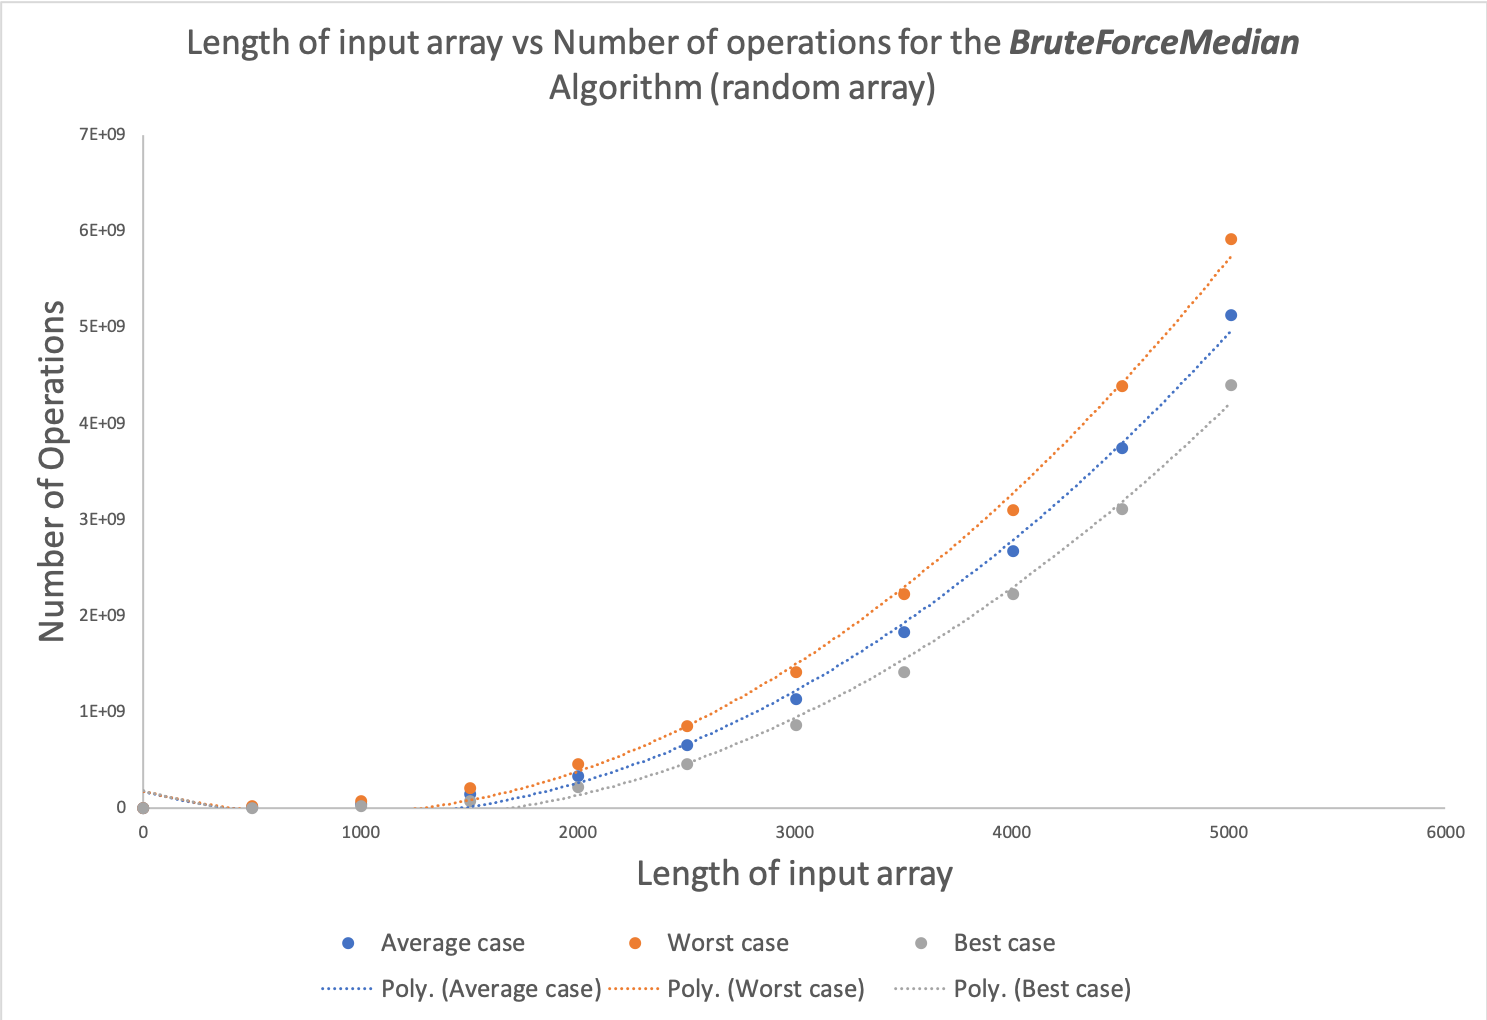
\includegraphics[width=0.9\linewidth]{Results/OpsRandom}
	\caption{Random array size of random elements vs the operational count.}
	\label{fig:opsrandom}
\end{figure}


\subsubsection{Random array size of reversed sorted elements (REVERSED): }

\begin{figure}[H]
	\centering
	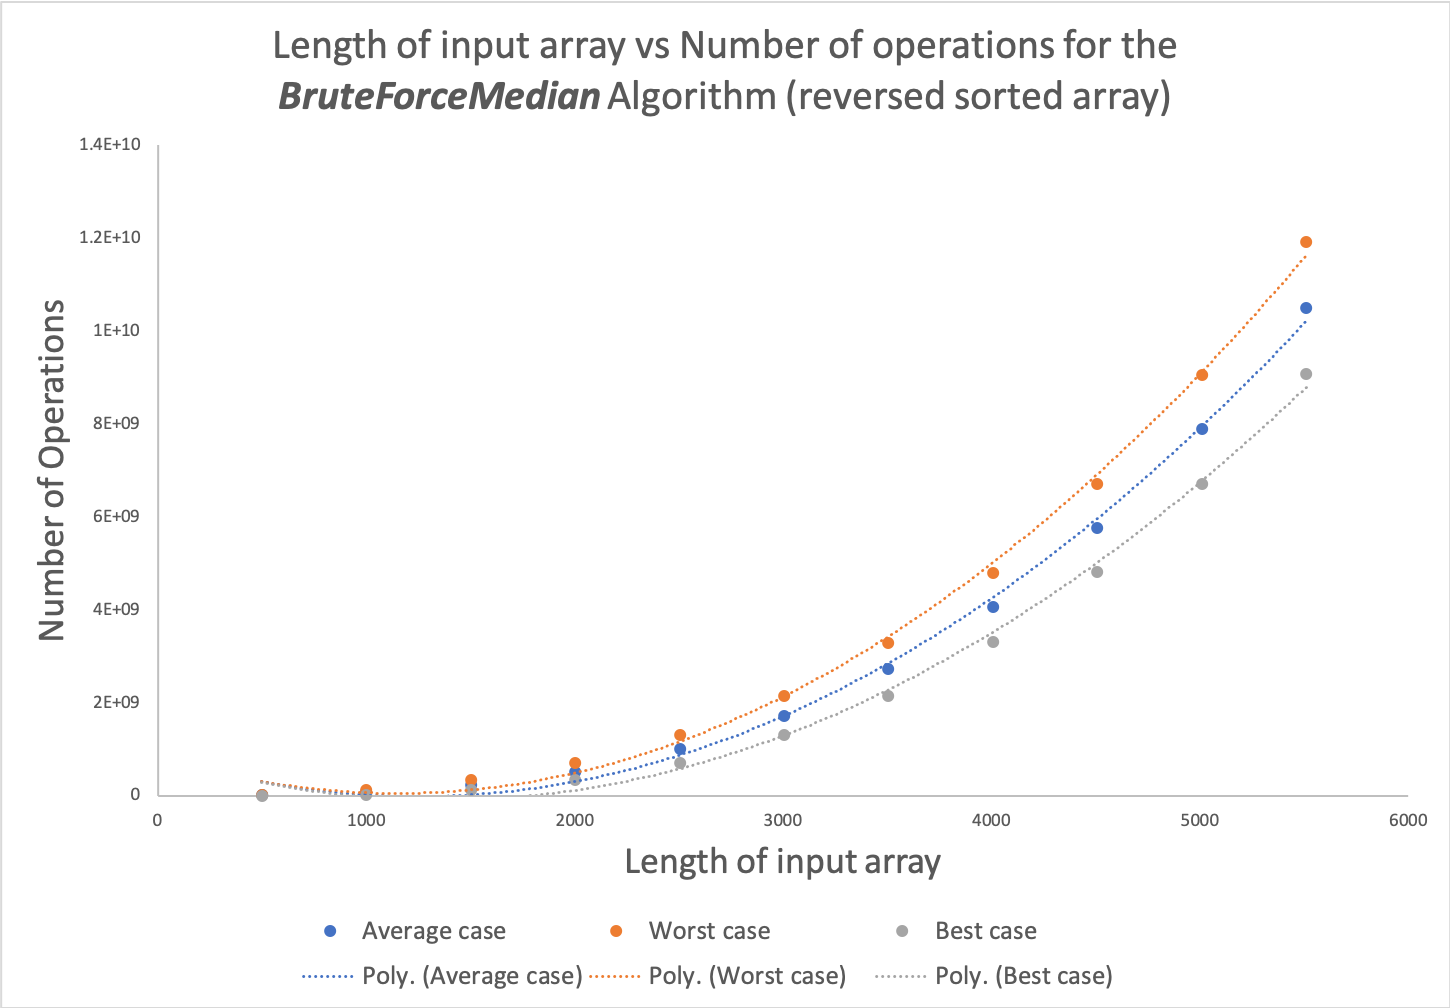
\includegraphics[width=0.9\linewidth]{Results/OpsReversed}
	\caption{Random array size of reversed sorted elements vs the operational count.}
	\label{fig:opsreversed}
\end{figure}


\subsubsection{Random array size of sorted elements (SORTED): }

\begin{figure}[H]
	\centering
	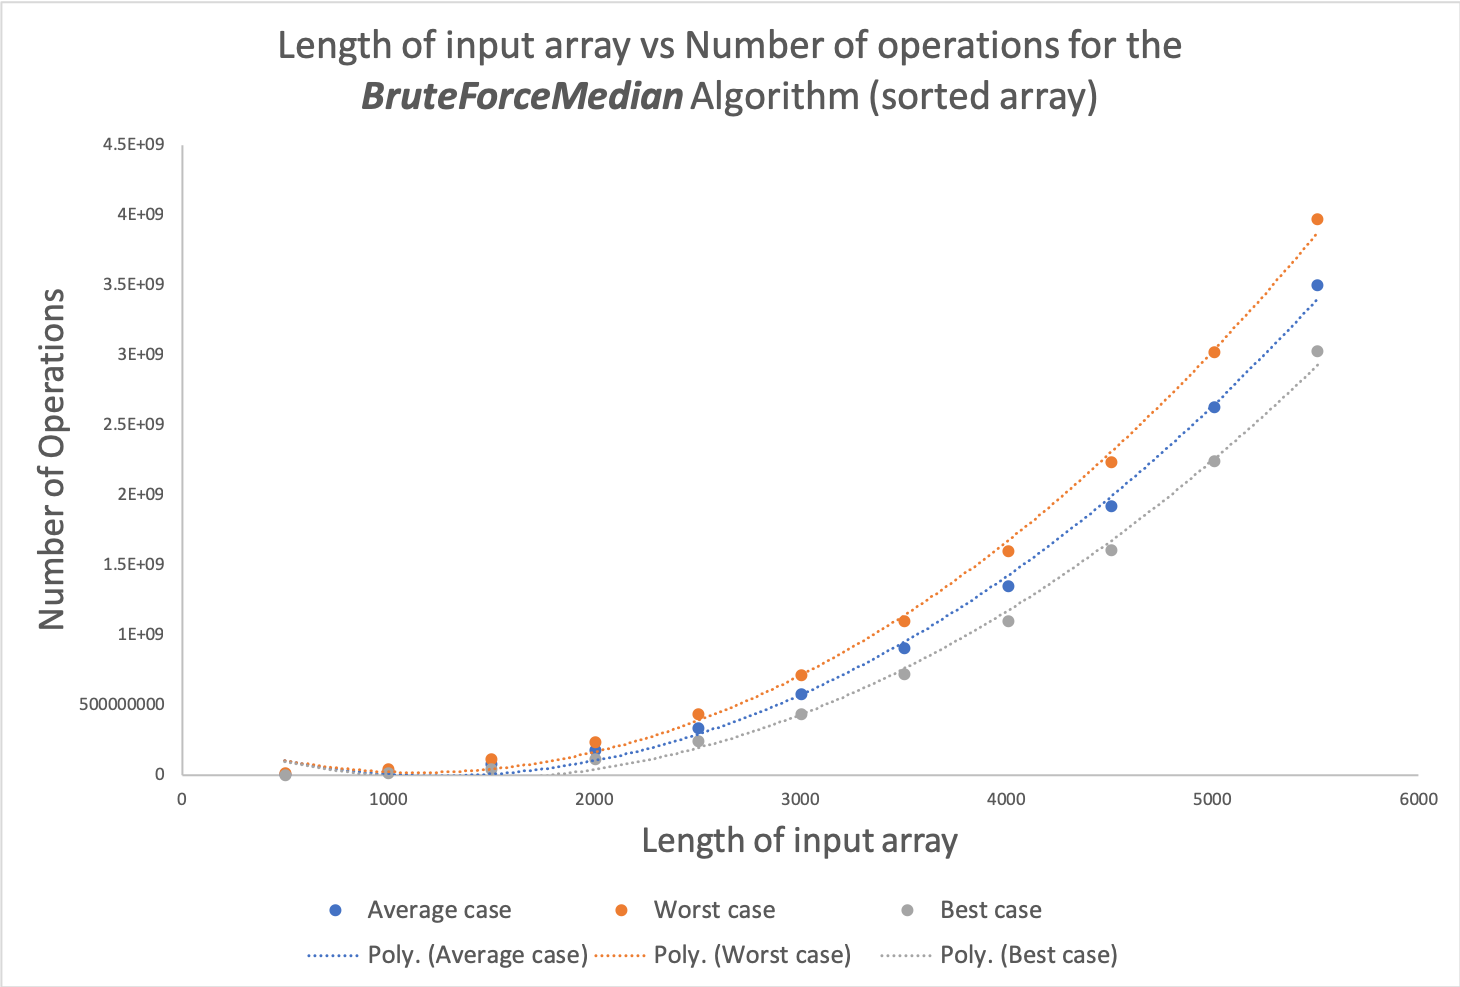
\includegraphics[width=0.9\linewidth]{Results/OpsSorted}
	\caption{Random array size of sorted elements vs the operational count.}
	\label{fig:opssorted}
\end{figure}

\subsection{Timing test results (graphs): }

\subsubsection{Random array size of random elements (RANDOM): }
\begin{figure}[H]
	\centering
	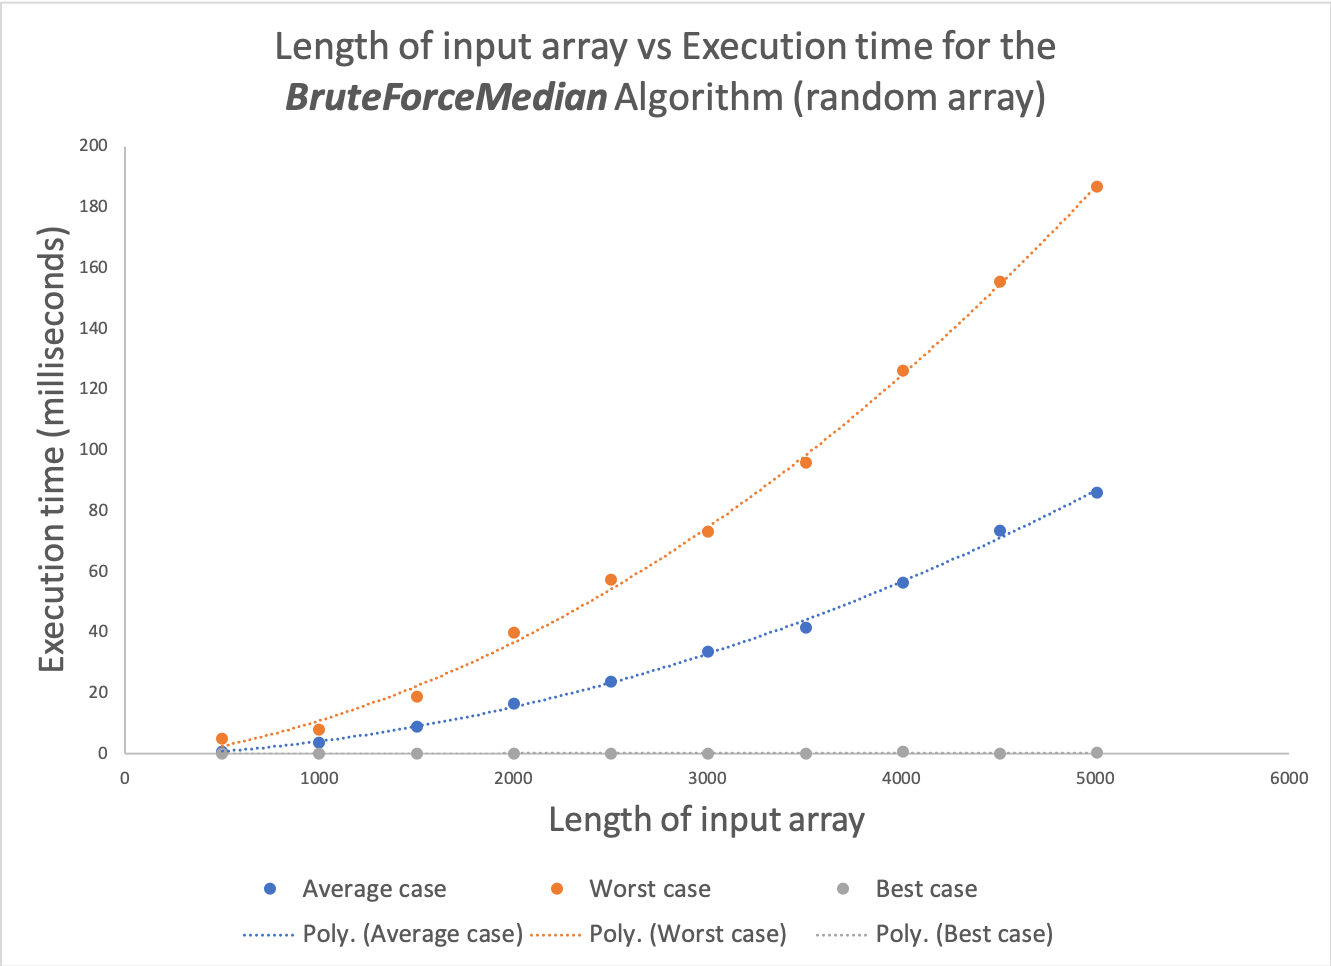
\includegraphics[width=0.9\linewidth]{Results/TimeRandom}
	\caption{Random array size of random elements vs the execution time of each test.}
	\label{fig:timerandom}
\end{figure}

\subsubsection{Random array size of reversed sorted elements (REVERSED): }


\begin{figure}[H]
	\centering
	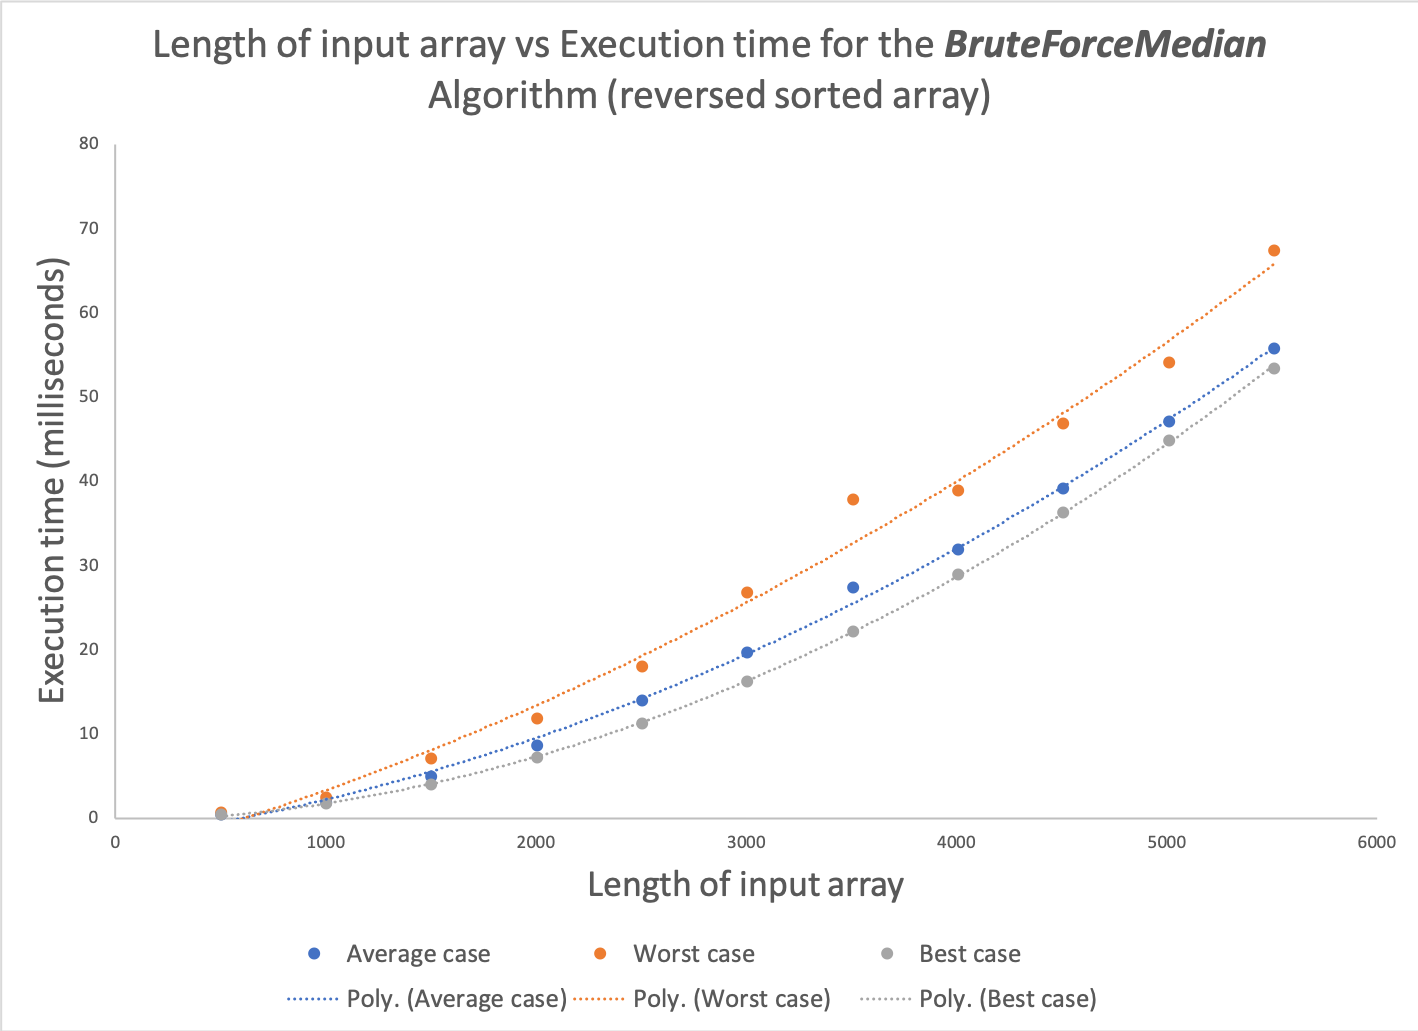
\includegraphics[width=0.9\linewidth]{Results/TimeReversed}
	\caption{Random array size of reversed sorted elements vs the execution time of each test.}
	\label{fig:timereversed}
\end{figure}


\subsubsection{Random array size of sorted elements (SORTED): }

\begin{figure}[H]
	\centering
	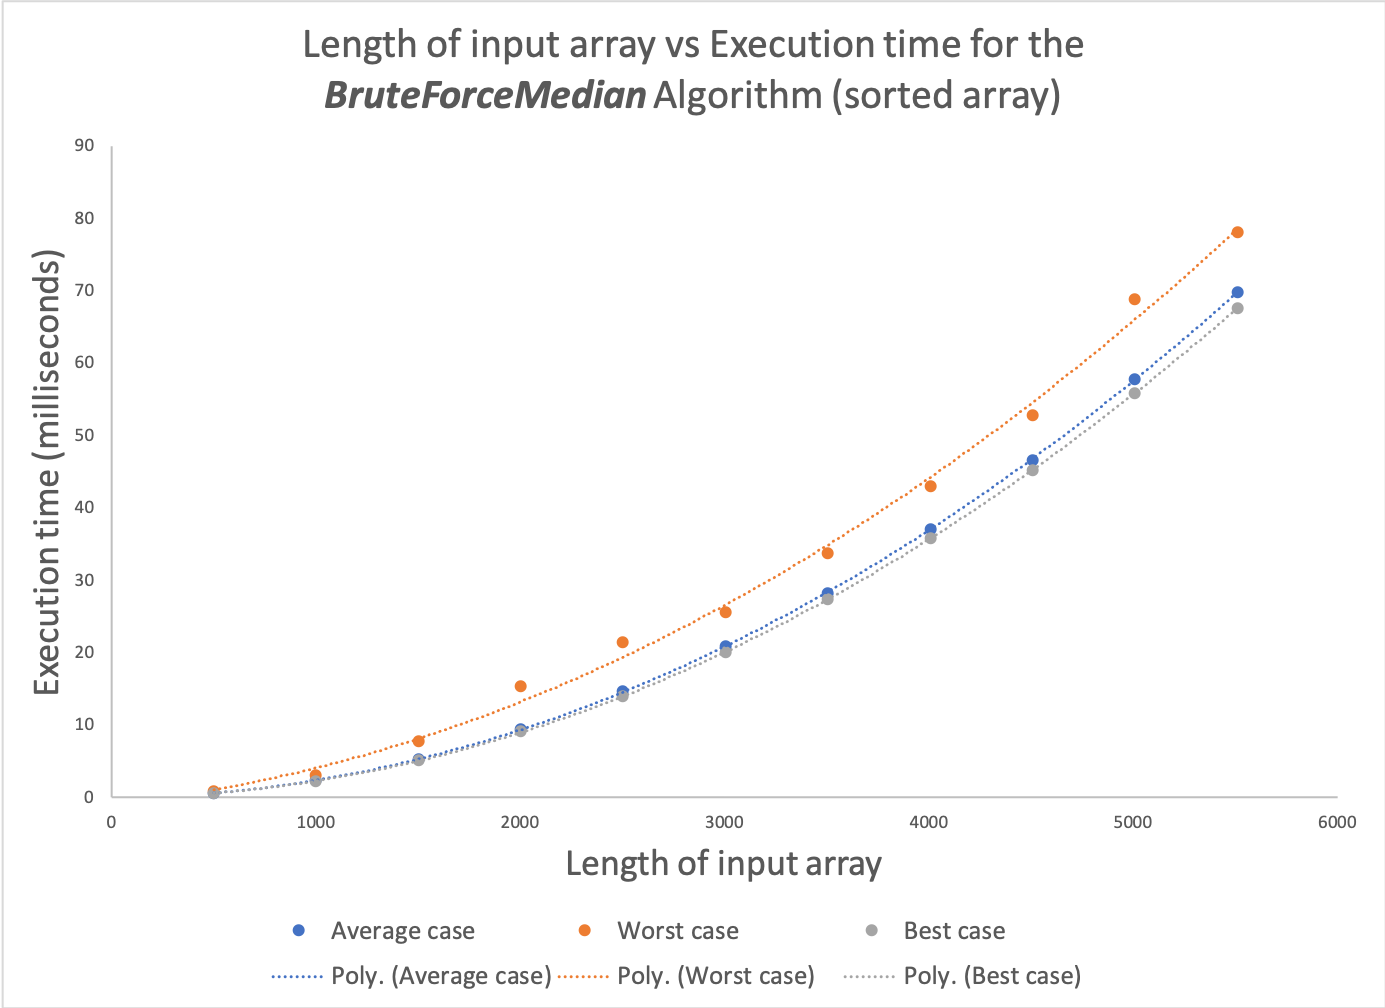
\includegraphics[width=0.9\linewidth]{Results/TimeSorted}
	\caption{Random array size of sorted elements vs the execution time of each test.}
	\label{fig:timesorted}
\end{figure}


\subsection{Comparison Algorithm}

\begin{lstlisting}[caption={Comparison algorithm used to compared the output from the \textbf{\textit{BruteForceMedian}} algorithm. Stored in the \textit{"comparisonAlgorithm.cpp" file.}},label={lst:comparison},language=C++,]
// sourced from - 
// https://stackoverflow.com/questions/2114797/compute-median-of-values-stored-in-vector-c/2114817#2114817
#include "headerFile.h"

int testMedian(vector<int> &input)
{
	// Storing the sorted vector in the local scope
	vector<int> sortedVect(input); 
	// Sort the vector
	sort(sortedVect.begin(), sortedVect.end());
	// Storing the size of the vector in size_t (basically an unsigned int)
	size_t size = sortedVect.size(); 
	if(size == 0)
	{
		return 0; // This is the null case when the array is 0;
	}else{
		sort(input.begin(), input.end()); // Sorting the vector
		// Checking condition of an even array
		// If is is an even array:
		// We return the element which is half the array size + 1 divided by two
		// If it is not an even array:
		// We return the element which is indexed as  half of the size of the array
		return size % 2 == 0 ? ceil((input[size / 2.0 - 1] + input[size / 2.0]) / 2.0) : input[size / 2];
	}
}

\end{lstlisting}

\subsection{BruteForceMedian Implementation:}

\begin{lstlisting}[caption={BruteForceMedian algorithm implementation for the number of operations, stored in the \textit{algorithmOps.cpp} file.},label={lst:bruteforceops},language=C++,]
#include "headerFile.h"

unsigned long long numOp = 0;

int BruteForceMedian(vector<int> &A)
{
	size_t size = A.size(); // Calculating the size fo the input array
	int k = (int) ceil(A.size() / 2.0); // Calculate the half-way index of the array.
	
	for (int i = 0; i <= (size-1); i++) {
		int numSmaller = 0; // Number of elements smaller than A[i];
		int numEqual = 0; // Number of elements equal to A[i];
		
		for (int j = 0; j <= (size-1); j++) {
			// Calculate number of array items that are smaller, and equal.
			if (A[j] < A[i]) {
			numSmaller+=1;
			numOp+=1;
			} else {
			if (A[j] == A[i]) {
			numEqual+=1;
			numOp+=1;
			}
		}
	}
	if ((numSmaller < k) && (k <= (numSmaller + numEqual))) {
			return A[i];
		}
	}
	return 0;
}

\end{lstlisting}


\subsection{Test Algorithms}

\begin{lstlisting}[language=C++, caption={Data generation algorithms - \textit{generateData.cpp} file}]
#include "headerFile.h"

vector<vector<int>> generateArray(TEST_TYPE type)
{
vector<vector<int>> outputArray;
vector<int> innerArray;
int Count = 0;
int random = 0;

srand(time(0));
switch (type) {
case NEGATIVE:
for (int i = 0; i < SIMULATIONS; i++)
{
for (int j = 0; j >= -((int) SIMULATIONS); j--)
{
innerArray.push_back(j);
}
outputArray.push_back(innerArray);
innerArray.clear();
}
break;
case ODD:
for (int i = 0; i < SIMULATIONS; i++)
{
for (int j = 1; j < (i*2)+2; j++)
{
innerArray.push_back(j);
}
outputArray.push_back(innerArray);
innerArray.clear();
}
break;
case EVEN:
for (int i = 0; i < SIMULATIONS; i++)
{
for (int j = 1; j < (i*2)+1; j++)
{
innerArray.push_back(j);
}
outputArray.push_back(innerArray);
innerArray.clear();
}
break;
case LARGE:
for (int i = 0; i < LARGE_ARRAY_SIMS; i++)
{
for (int j = 1; j < LARGE_ARRAY_VALUE; j++)
{
innerArray.push_back(j);
}
outputArray.push_back(innerArray);
innerArray.clear();
}
break;
case ONELEN:
for (int i = 0; i < SIMULATIONS; i++)
{
for (int j = 1; j <= 1; j++)
{
innerArray.push_back(j);
}
outputArray.push_back(innerArray);
innerArray.clear();
}
break;

case NOLEN:
for (int i = 0; i < SIMULATIONS; i++)
{
outputArray.push_back(innerArray);
}
break;
case RANDOM:
for(int i = 0; i < SIMULATIONS; i++)
{
Count+=ARRAY_STEP_SIZE;
for(int j = 0;j < ARRAY_NUM_SIMS; j++)
{
for (int k = 0; k < Count; k++)
{
random = rand() % RANDOM_RANGE;
innerArray.push_back(random);
}
outputArray.push_back(innerArray);
innerArray.clear();

}
}
break;
case REVERSED:
for(int i = 0; i < (SIMULATIONS + 1); i++)
{
Count+=ARRAY_STEP_SIZE;
for(int j = 0;j < ARRAY_NUM_SIMS; j++)
{
for (int k = 0; k < Count; k++)
{
innerArray.push_back((int) ((Count) - k - 1));
}
outputArray.push_back(innerArray);
innerArray.clear();
}
}
break;
case SORTED:
for(int i = 0; i < (SIMULATIONS + 1); i++)
{
Count+=ARRAY_STEP_SIZE;
for(int j = 0;j < ARRAY_NUM_SIMS; j++)
{
for (int k = 0; k < Count; k++)
{
innerArray.push_back(k);
}
outputArray.push_back(innerArray);
innerArray.clear();
}
}
break;

}
return outputArray;
}

\end{lstlisting}

\subsection{Program Implementation:}

\begin{table}[H]
	\centering
	\caption{Preprocessor variable names and their definitions defined in the \textit{headerFile.h}}
	\label{tab:preprocessordirectives}
	\resizebox{\textwidth}{!}{%
		\begin{tabular}{lL{0.65\textwidth}llll}
			\textbf{Variable Name} & \textbf{Definition} & \textbf{Related Test} &  &  \\ \cline{1-3}
			LARGE\_ARRAY\_VALUE & This is the variable which is used for the large array test. & LARGE ARRAY &  &  \\ \cline{1-3}
			LARGE\_ARRAY\_SIMS & This is the amount of simulations performed for the large array test (DEFAULT 1). & LARGE ARRAY &  &  \\ \cline{1-3}
			ARRAY\_STEP\_SIZE & Step size for the random array test. & RANDOM ARRAY &  &  \\ \cline{1-3}
			ARRAY\_NUM\_SIMS & Number of the same length arrays for the random array test. & RANDOM ARRAY &  &  \\ \cline{1-3}
			RANDOM\_RANGE & Range for the random number generation for the random array test. & RANDOM ARRAY &  &  \\ \cline{1-3}
			SIMULATIONS & Number of simulations performed by the program. & ALL TESTS &  & 
		\end{tabular}%
	}
\end{table}

\begin{figure}[H]
	\centering
	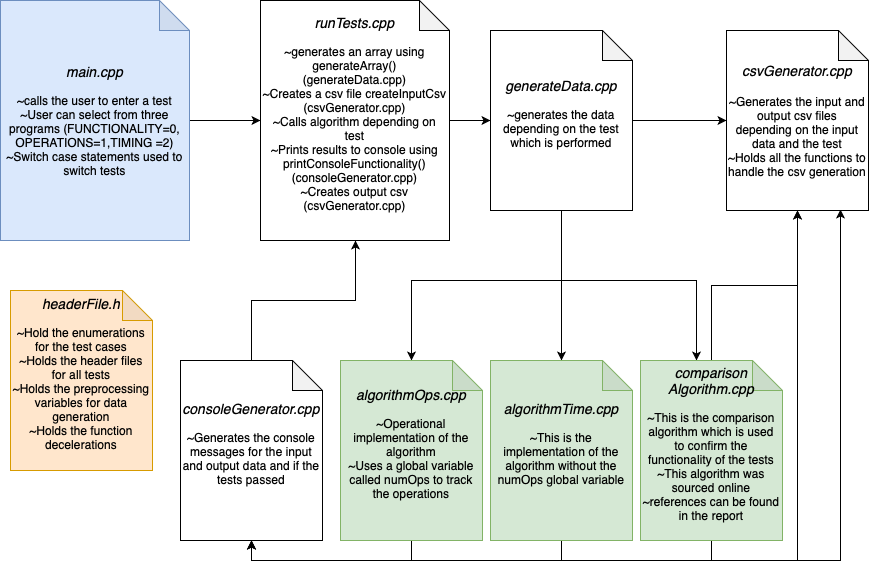
\includegraphics[width=1\linewidth]{Results/ProgramOverview}
	\caption{Top down ovevrview of the program implementation.}
	\label{fig:programoverview}
\end{figure}




\end{document}          
